%!TEX root = da-screen.tex

Imagine that we have $n$ computers that are connected to each other with communication channels so that the network topology is a \emph{path}:
\begin{center}
    \includegraphics[page=\PIntroTopo]{figs.pdf}
\end{center}
Our task is to find a proper \emph{colouring} of the path with $3$ colours. That is, each computer has to output one of the colours, $1$, $2$, or $3$, so that neighbours have different colours:
\begin{center}
    \includegraphics[page=\PIntroCol]{figs.pdf}
\end{center}

\section{Colouring with Distributed Algorithm}

With a bird's-eye view of the entire network, colouring a path looks like a very simple task: just start from one endpoint and assign colours $1$ and $2$ alternatingly. However, in a real-world computer network we usually do not have all-powerful entities that know everything about the network and can directly tell each computer what to do.

Indeed, when we start a networked computer, it is typically only aware of itself and the communication channels that it can use. In our simple example, the endpoints of the path know that they have one neighbour:
\begin{center}
    \includegraphics[page=\PIntroDegOne]{figs.pdf}
\end{center}
All other nodes along the path just know that they have two neighbours:
\begin{center}
    \includegraphics[page=\PIntroDegTwo]{figs.pdf}
\end{center}
For example, the second node along the path looks no different from the third node, yet somehow they have to produce \emph{different} outputs.

Obviously, the nodes have to exchange \emph{messages} with each other in order to figure out a proper solution. Yet this turns out to be surprisingly difficult even in the case of just $n = 2$ nodes:
\begin{center}
    \includegraphics[page=\PIntroTwo]{figs.pdf}
\end{center}
If we have two \emph{identical} computers connected to each other with a single communication link, both computers are started simultaneously, and both of them run the same deterministic algorithm, how could they ever end up in \emph{different} states?

As we will see in Chapter~\ref{ch:intro-neg}, the answer is that it is not possible, without some additional assumptions. In practice, we could try to rely on some imperfections (e.g., the computers are seldom perfectly synchronised), but in the theory of distributed algorithms we often assume that there is some explicit way to \emph{break symmetry} between otherwise identical computers. In this chapter, we will have a brief look at two common assumption:
\begin{itemize}[noitemsep]
    \item each computer has a unique name (Section~\ref{sec:intro-pos-id}),
    \item the computers can use randomness (Section~\ref{sec:intro-pos-random}).
\end{itemize}
In subsequent chapters we will then formalise these models, and develop a theory that will help us understand precisely what kind of tasks can be solved in each case, and how fast.


\section{Colouring with Unique Identifiers}\label{sec:intro-pos-id}

There are plenty of examples of real-world networks with globally unique identifiers: public IPv4 and IPv6 addresses are globally unique identifiers of Internet hosts, devices connected to an Ethernet network have globally unique MAC addresses, mobile phones have their IMEI numbers, etc. The common theme is that the identifiers are (supposed to be) globally unique, and the numbers can be interpreted as natural numbers:
\begin{center}
    \includegraphics[page=\PIntroId]{figs.pdf}
\end{center}
FIXME: Greedy graph colouring. Cole--Vishkin graph colouring.

\section{Colouring with Randomised Algorithms}\label{sec:intro-pos-random}

FIXME
